\chapter{Gravitational Instability and Collapse}
\label{ch:collapse}

\marginnote{
\textbf{Suggested background reading:}
\begin{itemize}
\item \href{http://adsabs.harvard.edu/abs/2014arXiv1402.0867K}{Krumholz, M.~R. 2014, Phys.~Rep., 539, 49}, section 3.4 \nocite{krumholz14c}
\end{itemize}
}

The previous two chapters provided a whirlwind tour of fluid dynamics and turbulence. However, in that discussion we completely omitted gravity, which is obviously critical to the process of star formation. We will now remedy that omission by bringing gravity back into the discussion.

\section{The Virial Theorem}

To open this topic, we will start by proving a powerful and general theorem about the behavior of fluids, known as the virial theorem.\footnote{Like the equations of motion, there is both an Eulerian form and a Lagrangian form of the virial theorem, depending on which version of the equations of motion we start with. We will derive the Eulerian form here, following the original proof by \citet{mckee92a}, but the derivation of the Lagrangian form proceeds in a similar manner, and can be found in many standard textbooks, for example \citet{shu92a}.} To derive the virial theorem, we begin with the MHD equations of motion, without either viscosity or resistivity (since neither of these are important for GMCs on large scales) but with gravity. We leave in the pressure forces, even though they are small, because they are also trivial to include. Thus we have
\begin{eqnarray}
\frac{\partial\rho}{\partial t} & = & -\nabla \cdot (\rho \vecv) \\
\frac{\partial}{\partial t}(\rho \vecv) & = & -\nabla\cdot(\rho\vecv\vecv) -\nabla P + \frac{1}{4\pi} (\nabla\times\vecB)\times\vecB - \rho \nabla \phi.
\end{eqnarray}
Here $\phi$ is the gravitational potential, so $-\rho \nabla \phi$ is the gravitational force per unit volume. These equations are the Eulerian equations written in conservative form.

Before we begin, life will be a bit easier if we re-write the entire second equation in a manifestly tensorial form -- this simplifies the analysis tremendously. To do so, we define two tensors: the fluid pressure tensor $\vecPi$ and the Maxwell stress tensor $\vecT_M$, as follows:
\begin{eqnarray}
\vecPi & \equiv & \rho \vecv\vecv + P\vecI \\
\vecT_M & \equiv & \frac{1}{4\pi} \left(\vecB\vecB - \frac{B^2}{2}\vecI\right)
\end{eqnarray}
Here $\vecI$ is the identity tensor. In tensor notation, these are
\begin{eqnarray}
(\vecPi)_{ij} & \equiv & \rho v_i v_j + P \delta_{ij} \\
(\vecT_M)_{ij} & \equiv & \frac{1}{4\pi} \left(B_i B_j - \frac{1}{2}B_k B_k \delta_{ij}\right).
\end{eqnarray}
With these definitions, the momentum equation just becomes
\begin{equation}
\frac{\partial}{\partial t}(\rho \vecv) = -\nabla\cdot(\vecPi-\vecT_M) - \rho \nabla\phi.
\end{equation}

The substitution for $\vecPi$ is obvious. The equivalence of $\nabla\cdot\vecT_M$ to $1/(4\pi) (\nabla\times\vecB)\times\vecB$ is easy to establish with a little vector manipulation, which is most easily done in tensor notation:
\begin{eqnarray}
(\nabla\times\vecB)\times\vecB & = & \epsilon_{ijk} \epsilon_{jmn} \left(\frac{\partial}{\partial x_m}B_n\right) B_k \\
& = & -\epsilon_{jik} \epsilon_{jmn} \left(\frac{\partial}{\partial x_m}B_n\right) B_k \\
& = & (\delta_{in}\delta_{km}-\delta_{im}\delta_{kn})\left(\frac{\partial}{\partial x_m}B_n\right) B_k \\
& = & B_k\frac{\partial}{\partial x_k} B_i - B_k\frac{\partial}{\partial x_i} B_k \\
& = & \left(B_k\frac{\partial}{\partial x_k} B_i + B_i \frac{\partial}{\partial x_k} B_k\right) - B_k\frac{\partial}{\partial x_i} B_k \\
& = & \frac{\partial}{\partial x_k}\left(B_i B_k\right) -\frac{1}{2} \frac{\partial}{\partial x_i} \left(B_k^2\right)\\
& = & \nabla\cdot \left(\vecB\vecB - \frac{B^2}{2}\vecI\right).
\end{eqnarray}

To derive the virial theorem, we begin by imagining a cloud of gas enclosed by some fixed volume $V$. The surface of this volume is $S$. We want to know how the overall distribution of mass changes within this volume, so we begin by writing down a quantity the represents the mass distribution. This is the moment of inertia,
\begin{equation}
I = \int_V \rho r^2\, dV.
\end{equation}

We want to know how this changes in time, so we take its time derivative:
\begin{eqnarray}
\dot{I} & = & \int_V \frac{\partial\rho}{\partial t} r^2 \,dV \\
& = & -\int_V \nabla \cdot (\rho \vecv) r^2\, dV \\
& = & -\int_V \nabla \cdot (\rho \vecv r^2)\, dV + 2\int_V \rho \vecv\cdot \vecr\, dV \\
& = & -\int_S (\rho \vecv r^2)\cdot d\vecS + 2\int_V \rho \vecv\cdot \vecr\, dV.
\end{eqnarray}
In the first step we used the fact that the volume $V$ does not vary in time to move the time derivative inside the integral. Then in the second step we used the equation of mass conservation to substitute. In the third step we brought the $r^2$ term inside the divergence. Finally in the fourth step we used the divergence theorem to replace the volume integral with a surface integral.

Now we take the time derivative again, and multiply by $1/2$ for future convenience:
\begin{eqnarray}
\frac{1}{2}\ddot{I} & = & -\frac{1}{2} \int_S r^2 \frac{\partial}{\partial t}(\rho\vecv)\cdot d\vecS +
\int_V \frac{\partial}{\partial t}(\rho\vecv)\cdot\vecr \, dV \\
& = & -\frac{1}{2} \frac{d}{dt} \int_S r^2 (\rho\vecv)\cdot d\vecS 
\nonumber \\
& & \quad {} -
\int_V \vecr \cdot \left[\nabla\cdot(\vecPi-\vecT_M)+ \rho\nabla \phi \right] \, dV.
\end{eqnarray}
The term involving the tensors is easy to simplify using a handy identity, which applies to an arbitrary tensor. This is a bit easier to follow in tensor notation:
\begin{eqnarray}
\int_V \vecr\cdot \nabla\cdot \vecT \, dV & = & \int_V x_i \frac{\partial}{\partial x_j} T_{ij}\,dV \\
& = & \int_V \frac{\partial}{\partial x_j}(x_i T_{ij})\,dV - \int_V T_{ij} \frac{\partial}{\partial x_j}x_i \, dV \\
& = & \int_S x_i T_{ij} \,dS_j - \int_V \delta_{ij} T_{ij} \, dV \\
& = & \int_S \vecr\cdot\vecT\cdot d\vecS - \int_V \mbox{Tr}\; \vecT \, dV,
\end{eqnarray}
where $\mbox{Tr}\;\vecT = T_{ii}$ is the trace of the tensor $\vecT$.

Applying this to our result our tensors, we note that
\begin{eqnarray}
\mbox{Tr}\; \vecPi & = & 3P + \rho v^2 \\
\mbox{Tr}\; \vecT_M & = & -\frac{B^2}{8\pi}
\end{eqnarray}
Inserting this result into our expression for $\ddot{I}$ gives the virial theorem, which we will write in a more suggestive form to make its physical interpretation clearer:
\begin{equation}
\frac{1}{2}\ddot{I} = 2(\mathcal{T} - \mathcal{T}_S) + \mathcal{B} + \mathcal{W} - \frac{1}{2}\frac{d}{dt} \int_S (\rho\vecv r^2)\cdot d\vecS,
\end{equation}
where
\begin{eqnarray}
\mathcal{T} & = & \int_V\left(\frac{1}{2}\rho v^2 + \frac{3}{2} P\right)\, dV \\
\mathcal{T}_S & = & \int_S \vecr \cdot \vecPi \cdot d\vecS\\
\mathcal{B} & = & \frac{1}{8\pi} \int_V B^2 \,dV + \int_S \vecr\cdot \vecT_M\cdot d\vecS\\
\mathcal{W} & = & -\int_V \rho \vecr\cdot\nabla\phi\,dV.
\end{eqnarray}

Written this way, we can give a clear interpretation to what these terms mean. $\mathcal{T}$ is just the total kinetic plus thermal energy of the cloud. $\mathcal{T}_S$ is the confining pressure on the cloud surface, including both the thermal pressure and the ram pressure of any gas flowing across the surface. $\mathcal{B}$ is the the difference between the magnetic pressure in the cloud interior, which tries to hold it up, and the magnetic pressure plus magnetic tension at the cloud surface, which try to crush it. $\mathcal{W}$ is the gravitational energy of the cloud. If there is no external gravitational field, and $\phi$ comes solely from self-gravity, then $\mathcal{W}$ is just the gravitational binding energy. The final integral represents the rate of change of the momentum flux across the cloud surface.

$\ddot{I}$ is the integrated form of the acceleration. For a cloud of fixed shape, it tells us the rate of change of the cloud's expansion or contraction. If it is negative, the terms that are trying to collapse the cloud (the surface pressure, magnetic pressure and tension at the surface, and gravity) are larger, and the cloud accelerates inward. If it is positive, the terms that favor expansion (thermal pressure, ram pressure, and magnetic pressure) are larger, and the cloud accelerates outward. If it is zero, the cloud neither accelerates nor decelerates.

We get a particularly simple form of the virial theorem if there is no gas crossing the cloud surface (so $\vecv=0$ at $S$) and if the magnetic field at the surface to be a uniform value $B_0$. In this case the virial theorem reduces to
\begin{equation}
\frac{1}{2}\ddot{I} = 2(\mathcal{T} - \mathcal{T}_S) + \mathcal{B} + \mathcal{W}
\end{equation}
with
\begin{eqnarray}
\mathcal{T}_S & = & \int_S rP \,dS\\
\mathcal{B} & = & \frac{1}{8\pi} \int_V (B^2-B_0^2) \,dV.
\end{eqnarray}
For this simplified physical setup, $\mathcal{T}_S$ just represents the mean radius times pressure at the virial surface, and $\mathcal{B}$ just represents the total magnetic energy of the cloud minus the magnetic energy of the background field over the same volume. Notice that, if a cloud is in equilibrium ($\ddot{I}=0$) and magnetic and surface forces are negligible, then we have $2\mathcal{T} = -\mathcal{W}$. Based on this result, we define the virial ratio
\begin{equation}
\label{eq:alpha_vir_th}
\alpha_{\rm vir} = \frac{2\mathcal{T}}{|\mathcal{W}|}.
\end{equation}
For an object for which magnetic and surface forces are negligible, and with no flow across the virial surface, a value of $\alpha_{\rm vir} > 1$ implies $\ddot{I} > 0$, and a value $\alpha_{\rm vir} < 1$ implies $\ddot{I}<0$. Thus $\alpha_{\rm vir} = 1$ roughly divides clouds that have enough internal pressure or turbulence to avoid collapse from those that do not.

\section{Stability Conditions}

Armed with the virial theorem, we are now in a position to understand, at least qualitatively, under what conditions a cloud of gas will be stable against gravitational contraction, and under what conditions it will not be. If we examine the terms on the right hand side of the virial theorem, we can group them into those that are generally or always positive, and thus oppose collapse, and those that are generally or always negative, and thus encourage it. The main terms opposing collapse are $\mathcal{T}$, which contains parts describing both thermal pressure and turbulent motion, and $\mathcal{B}$, which describes magnetic pressure and tension. The main terms favoring collapse are $\mathcal{W}$, representing self-gravity, and $\mathcal{T}_S$, representing surface pressure. The final term, the surface one, could be positive or negative depending on whether mass is flowing into our out of the virial volume. We will begin by examining the balance among these terms, and the forces they represent.

\subsection{Thermal Support and the Jeans Instability}

Gas pressure is perhaps the most basic force in opposing collapse. Unlike turbulent motions, which can compress in some places even as they provide overall support, gas pressure always tries to smooth out the gas. Similarly, self-gravity is the most reliable promoter of collapse. A full, formal analysis of the interaction between pressure and self-gravity was provided by James Jeans in 1902 \citep{jeans02a}, and we will go through it below. However, we can already see what the basic result will have to look like just from the virial theorem. We expect the dividing line between stability and instability to lie at $\alpha_{\rm vir} \approx 1$. For an isolated, isothermal cloud of mass $M$ and radius $R$ with only thermal pressure, we have
\begin{eqnarray}
\mathcal{T} & = & \frac{3}{2} M c_s^2 \\
\mathcal{W} & = & -a \frac{GM^2}{R},
\end{eqnarray}
where $a$ is a factor of order unity that depends on the internal density structure. Thus the condition $\alpha_{\rm vir} \gtrsim 1$ corresponds to
\begin{equation}
M c_s^2 \gtrsim \frac{GM^2}{R} \qquad\Longrightarrow\qquad R \gtrsim \frac{GM}{c_s^2},
\end{equation}
or, rewriting in terms of the mean density $\rho \sim M/R^3$,
\begin{equation}
R \gtrsim \frac{c_s}{\sqrt{G\rho}}.
\end{equation}

The formal analysis proceeds as follows. Consider a uniform, infinite, isothermal medium at rest. The density is $\rho_0$, the pressure is $P_0 = \rho_0 c_s^2$, and the velocity is $\vecv_0 = 0$. We will write down the equations of hydrodynamics and self-gravity for this gas:
\begin{eqnarray}
\frac{\partial}{\partial t}\rho + \nabla\cdot (\rho \vecv) & = & 0 \\
\frac{\partial}{\partial t}(\rho\vecv) + \nabla\cdot(\rho \vecv\vecv) & = & -\nabla P - \rho \nabla \phi \\
\nabla^2 \phi & = & 4\pi G\rho.
\end{eqnarray}

Here the first equation represents conservation of mass, the second represents conservation of momentum, and the third is the Poisson equation for the gravitational potential $\phi$. We take the background density $\rho_0$, velocity $\vecv_0 = 0$, pressure $P_0$, and potential $\phi_0$ to be an exact solution of these equations, so that all time derivatives are zero as long as the gas is not disturbed.

Note that this involves the "Jeans swindle": this assumption is actually not really consistent, because the Poisson equation cannot be solved for an infinite uniform medium unless $\rho_0 = 0$. In other words, there is no function $\phi_0$ such that $\nabla^2\phi_0$ is equal to a non-zero constant value on all space. That said, we will ignore this complication, since the approximation of a uniform infinite medium is a reasonable one for a very large but finite uniform medium. It is possible to construct the argument without the Jeans swindle, but doing so adds mathematical encumbrance without physical insight, so we will not do so.

That digression aside, now let us consider what happens if we perturb this system. We will write the density as $\rho = \rho_0 + \epsilon \rho_1$, where $\epsilon\ll 1$. Similarly, we write $\vecv=\epsilon \vecv_1$ and $\phi=\phi_0 + \epsilon \phi_1$. Since we can always use Fourier analysis to write an arbitrary perturbation as a sum of Fourier components, without loss of generality we will take the perturbation to be a single, simple Fourier mode. The reason to do this is that, as we will see, differential equations are trivial to solve when the functions in question are simple plane waves.

Thus we write $\rho_1 = \rho_a \exp[i(kx - \omega t)]$. Note that we implicitly understand that we use only the real part of this exponential. It is just easier to write things in terms of an $e^{i(kx-\omega t)}$ than it is to keep track of a bunch of sines and cosines. In writing this equation, we have chosen to orient our coordinate system so that the wave vector $\veck$ of the perturbation is in the $\vecx$ direction. Again, there is no loss of generality in doing so.

Given this density perturbation, what is the corresponding perturbation to the potential? From the Poisson equation, we have
\begin{equation}
\nabla^2 (\phi_0 + \epsilon \phi_1) = 4\pi G (\rho_0 + \epsilon \rho_1).
\end{equation}
Since by assumption $\rho_0$ and $\phi_0$ are exact solutions to the Poisson equation, we can cancel the $\phi_0$ and $\rho_0$ terms out of the equation, leaving
\begin{equation}
\nabla^2 \phi_1 = 4 \pi G \rho_1 = 4\pi G \rho_a e^{i(kx-\omega t)}.
\end{equation}
This equation is trivial to solve, since it is just of the form $y'' = a e^{bx}$. The solution is
\begin{equation}
\phi_1 = -\frac{4\pi G \rho_a}{k^2} e^{i(kx - \omega t)}.
\end{equation}
By analogy to what we did for $\rho_1$, we write this solution as $\phi_1 = \phi_a e^{i(kx-\omega t)}$, with
\begin{equation}
\phi_a = -\frac{4\pi G \rho_a}{k^2}.
\end{equation}

Now that we have found the perturbed potential, let us determine what motion this will induce in the fluid. To do so, we first take the equations of mass and momentum conservation and we linearize them. This means that we substitute in $\rho = \rho_0 + \epsilon \rho_1$, $\vecv=\epsilon \vecv_1$, $P=P_0+\epsilon P_1=c_s^2 (\rho_0 + \epsilon \rho_1)$, and $\phi=\phi_0+\epsilon \phi_1$. Note that $\vecv_0 = 0$. We then expand the equations in powers of $\epsilon$, and we drop all the terms that are of order $\epsilon^2$ or higher on the grounds that they become negligible in the limit of small $\epsilon$.

Linearizing the equation of mass conservation we get
\begin{eqnarray}
\frac{\partial}{\partial t} (\rho_0 + \epsilon \rho_1) + \nabla\cdot [(\rho_0 + \epsilon \rho_1)(\epsilon\vecv_1)] & = & 0 \\
\frac{\partial}{\partial t} \rho_0 + \epsilon \frac{\partial}{\partial t} \rho_1 + \epsilon \nabla \cdot (\rho_0\vecv_1) & = & 0 \\
\frac{\partial}{\partial t} \rho_1+ \nabla \cdot (\rho_0\vecv_1) & = & 0.
\label{eq:masscons_linear}
\end{eqnarray}
In the second step, we dropped a term of order $\epsilon^2$. In the third step we used the fact that $\rho_0$ is constant, i.e., that the background density has zero time derivative, to drop that term. Applying the same procedure to the momentum equation, we get
\begin{eqnarray}
\nonumber
\lefteqn{
\frac{\partial}{\partial t} [(\rho_0 + \epsilon \rho_1)(\epsilon\vecv_1)] + \nabla\cdot [(\rho_0 + \epsilon \rho_1)(\epsilon\vecv_1)(\epsilon\vecv_1)] 
}
\qquad\qquad\qquad
\\
& = & -c_s^2 \nabla (\rho_0 + \epsilon \rho_1) \nonumber \\
& & \qquad {} - (\rho_0 + \epsilon\rho_1)\nabla (\phi_0 + \epsilon \phi_1)
\\
\epsilon \frac{\partial}{\partial t} (\rho_0\vecv_1) & = & -c_s^2 \nabla \rho_0 - \rho_0 \nabla\phi_0
\nonumber \\
& & \qquad {}
- \epsilon \left(c_s^2 \nabla \rho_1 + \rho_1\nabla \phi_0 + \rho_0\nabla \phi_1\right) \\
\frac{\partial}{\partial t} (\rho_0\vecv_1) & = & -c_s^2 \nabla \rho_1 - \rho_0\nabla\phi_1.
\label{eq:momcons_linear}
\end{eqnarray}
In the second step we dropped terms of order $\epsilon^2$, and in the third step we used the fact that the background state is uniform to drop terms involving gradients of $\rho_0$ and $\phi_0$.

Now that we have our linearized equations, we're ready to find out what $\vecv_1$ must be. By analogy to what we did for $\rho_1$ and $\phi_1$, we take $\vecv_1$ to be a single Fourier mode, of the form
\begin{equation}
\vecv_1 = \vecv_a e^{i(kx-\omega t)}
\end{equation}
Substituting for $\rho_1$, $\phi_1$, and $\vecv_1$ into the linearized mass conservation equation (\ref{eq:masscons_linear}), we get
\begin{eqnarray}
\frac{\partial}{\partial t} \left(\rho_a e^{i(kx-\omega t)}\right) + \nabla\cdot (\rho_0 \vecv_a e^{i(kx-\omega t)}) & = & 0 \\
-i\omega \rho_a e^{i(kx-\omega t)} + i k \rho_0 v_{a,x} e^{i(kx-\omega t)} & = & 0 \\
-\omega\rho_a + k\rho_0 v_{a,x} & = & 0 \\
\frac{\omega\rho_a}{k\rho_0} & = & v_{a,x}
\end{eqnarray}
where $v_{a,x}$ is the $x$ component of $\vecv_a$.

We have now found the velocity perturbation in terms of $\rho_a$, $\omega$, and $k$. Similarly substituting into the linearized momentum equation (\ref{eq:momcons_linear}) gives
\begin{eqnarray}
\frac{\partial}{\partial t} \left(\rho_0 \vecv_a e^{i(kx-\omega t)}\right) & = & -c_s^2 \nabla(\rho_a e^{i(kx-\omega t)})
\nonumber \\
& & \qquad {}
 - \rho_0 \nabla (\phi_a e^{i(kx-\omega t)}) \\
-i\omega \rho_0 \vecv_a e^{i(kx-\omega t)} & = & -i k c_s^2 \rho_a \hat{\mathbf{x}} e^{i(kx-\omega t)} 
\nonumber \\
& & \qquad {}
- i k \rho_0 \phi_a e^{i(kx-\omega t)} \hat{\mathbf{x}}\\
\omega \rho_0 v_{a,x} & = & k \left(c_s^2 \rho_a + \rho_0 \phi_a\right).
\end{eqnarray}
Now let us take this equation and substitute in the values for $\phi_a$ and $v_{a,x}$ that we previously determined:
\begin{eqnarray}
\omega \rho_0 \left(\frac{\omega\rho_a}{k\rho_0}\right) & = & k c_s^2 \rho_a - k\rho_0 \left(\frac{4\pi G \rho_a}{k^2}\right) \\
\omega^2 & = & c_s^2 k^2 - 4\pi G \rho_0
\end{eqnarray}
This expression is known as a dispersion relation, because it describes the dispersion of the plane wave solution we have found, i.e., how that wave's spatial frequency $k$ relates to its temporal frequency $\omega$. 

To see what this implies, let us consider what happens when we put in a perturbation with a short wavelength or a large spatial frequency. In this case $k$ is large, and $c_s^2 k^2 - 4\pi G \rho_0>0$, so $\omega$ is a positive or negative real number. The density is $\rho=\rho_0 + \rho_a e^{i(kx-\omega t)}$, which represents a uniform background density with a small oscillation in space and time on top of it. Since $|e^{i(kx-\omega t)}| < 1$ at all times and places, the oscillation does not grow.

On the other hand, suppose that we impose a perturbation with a large spatial range, or a small spatial frequency. In this case $c_s^2 k^2 - 4\pi G \rho_0<0$, so $\omega$ is a positive or negative imaginary number. For an imaginary $\omega$, $|e^{-i\omega t}|$ either decays to zero or grows infinitely large in time, depending on whether we take the positive or negative imaginary root. Thus at least one solution for the perturbation will not remain small. It will grown in amplitude without limit.

This represents an instability: if we impose an arbitrarily small amplitude perturbation on the density at a sufficiently large wavelength, that perturbation will eventually grow to be large. Of course once $\rho_1$ becomes large enough, our linearization procedure of dropping terms proportional to $\epsilon^2$ becomes invalid, since these terms are no longer small. In this case we must follow the full non-linear behavior of the equations, usually with simulations.

We have, however, shown that there is a critical size scale beyond which perturbations that are stabilized only by pressure must grow to non-linear amplitude. The critical length scale is set by the value of $k$ for which $\omega=0$,
\begin{equation}
k_J = \sqrt{\frac{4\pi G\rho_0}{c_s^2}}.
\end{equation}
The corresponding wavelength is
\begin{equation}
\lambda_J = \frac{2\pi}{k_J} = \sqrt{\frac{\pi c_s^2}{G\rho_0}}.
\end{equation}
This is known as the Jeans length. One can also define a mass scale associated with this: the Jeans mass, $M_J=\rho\lambda_J^3/8$.\footnote{The definition of the Jeans mass is somewhat ambiguous, and multiple definitions can be found in the literature. The one we have chosen corresponds to considering the mass within a cube of half a Jeans length in size. Possible alternatives include choosing a cube one Jeans length in size or choosing a sphere one Jeans length in radius or diameter, to name just two possibilities. These definitions all scale with density and Jeans length in the same way, and differ only in their coefficients.}

If we plug in some typical numbers for a GMC, $c_s=0.2$ km s$^{-1}$ and $\rho_0 = 100 m_p\mbox{ cm}^{-3}$, we get $\lambda_J = 3.4$ pc. Since every GMC we have seen is larger than this size, and there are clearly always perturbations present, this means that molecular clouds cannot be stabilized by gas pressure against collapse. Of course one could have guessed this result just by evaluating terms in the virial theorem: the gas pressure term is very small compared to the gravitational one. Ultimately, the virial theorem and the Jeans instability analysis are just two different ways of extracting the same information from the equations of motion.

One nice thing about the Jeans analysis, however, is that it makes it obvious how fast we should expect gravitational instabilities to grow. Suppose we have a very unstable system, where $c_s^2 k^2 \ll 4 \pi G \rho_0$. This is the case for GMC, for example. There are perturbations on the size of the entire cloud, which might be 50 pc in size. This is a spatial frequency $k=2\pi/(50\mbox{ pc}) = 0.12$ pc$^{-1}$. Plugging this in with $c_s = 0.2$ km s$^{-1}$ and $\rho_0=100 m_p\mbox{ cm}^{-3}$ gives $c_s^2 k^2 / (4\pi G \rho) = 0.005$.
In this case we have
\begin{equation}
\omega \approx \pm i \sqrt{4\pi G\rho_0}.
\end{equation}

Taking the negative $i$ root, which corresponds to the growing mode, we find that
\begin{equation}
\rho_1 \propto \exp([4\pi G \rho_0]^{1/2} t).
\end{equation}
Thus the $e$-folding time for the disturbance to grow is $\sim 1/\sqrt{G\rho_0}$. We define the free-fall time as
\begin{equation}
t_{\rm ff} = \sqrt{\frac{3\pi}{32 G \rho_0}},
\end{equation}
where the numerical coefficient of $\sqrt{3\pi/32}$ comes from doing the closely related problem of the collapse of a pressureless sphere, which we will cover in Section \ref{sec:pressureless_collapse}. The free-fall time is the characteristic time scale required for a medium with negligible pressure support to collapse.

The Jeans analysis is of course only appropriate for a uniform medium, and it requires the Jeans swindle. Problem Set 2 contains a calculation of the maximum mass of a spherical cloud that can support itself against collapse by thermal pressure, called the Bonnor-Ebert mass \citep{ebert55a, bonnor56a}. Not surprisingly, the Bonnor-Ebert mass is simply $M_J$ times factors of order unity.

\subsection{Magnetic Support and the Magnetic Critical Mass}

We now examine another term that generally opposes collapse: the magnetic one. Let us consider a uniform spherical cloud of radius $R$ threaded by a magnetic field $\vecB$. We imagine that $\vecB$ is uniform inside the cloud, but that outside the cloud the field lines quickly spread out, so that the magnetic field drops down to some background strength $\vecB_0$, which is also uniform but has a magnitude much smaller than $\vecB$.

Here it is easiest to work directly with the virial theorem. The magnetic term in the virial theorem is
\begin{equation}
\mathcal{B} = \frac{1}{8\pi} \int_V B^2 \,dV + \int_S \vecr \cdot \vecT_M \cdot d\vecS
\end{equation}
where
\begin{equation}
\vecT_M = \frac{1}{4\pi} \left(\vecB\vecB - \frac{B^2}{2}\vecI\right).
\end{equation}

If the field inside the cloud is much larger than the field outside it, then the first term, representing the integral of the magnetic pressure within the cloud, is
\begin{equation}
\frac{1}{8\pi} \int_V B^2\, dV \approx \frac{B^2 R^3}{6}.
\end{equation}
Here we have dropped any contribution from the field outside the cloud. The second term, representing the surface magnetic pressure and tension, is
\begin{equation}
\int_S \vecx \cdot \vecT_M \cdot d\vecS = \int_S \frac{B_0^2}{8\pi} \vecx \cdot d\vecS
\approx \frac{B_0^2 R_0^3}{6}
\end{equation}

Since the field lines that pass through the cloud must also pass through the virial surface, it is convenient to rewrite everything in terms of the magnetic flux. The flux passing through the cloud is $\Phi_B = \pi B R^2$, and since these field lines must also pass through the virial surface, we must have $\Phi_B = \pi B_0 R_0^2$ as well. Thus, we can rewrite the magnetic term in the virial theorem as
\begin{equation}
\mathcal{B} \approx \frac{B^2 R^3}{6} - \frac{B_0^2 R_0^3}{6} = \frac{1}{6\pi^2} \left(\frac{\Phi_B^2}{R} - \frac{\Phi_B^2}{R_0}\right) \approx \frac{\Phi_B^2}{6\pi^2 R}.
\end{equation}

In the last step we used the fact that $R \ll R_0$ to drop the $1/R_0$ term. Now let us compare this to the gravitational term, which is
\begin{equation}
\mathcal{W} = -\frac{3}{5} \frac{GM^2}{R}
\end{equation}
for a uniform cloud of mass $M$. Comparing these two terms, we find that
\begin{equation}
\mathcal{B}+\mathcal{W} = \frac{\Phi_B^2}{6\pi^2 R} - \frac{3}{5} \frac{GM^2}{R} \equiv \frac{3}{5}\frac{G}{R} \left(M_{\Phi}^2-M^2\right)
\end{equation}
where
\begin{equation}
\label{eq:mphi}
M_{\Phi} \equiv \sqrt{\frac{5}{2}} \left(\frac{\Phi_B}{3 \pi G^{1/2}}\right)
\end{equation}
We call $M_{\Phi}$ the magnetic critical mass. Since $\Phi_B$ does not change as a cloud expands or contracts (due to flux-freezing), this magnetic critical mass does not change either.

The implication of this is that clouds that have $M>M_{\Phi}$ always have $\mathcal{B}+\mathcal{W} < 0$. The magnetic force is unable to halt collapse no matter what. Clouds that satisfy this condition are called magnetically supercritical, because they are above the magnetic critical mass $M_{\Phi}$. Conversely, if $M<M_{\Phi}$, then $\mathcal{B}+\mathcal{W} > 0$, and gravity is weaker than magnetism. Clouds satisfying this condition are called subcritical.

For a subcritical cloud, since $\mathcal{B}+\mathcal{W} \propto 1/R$, this term will get larger and larger as the cloud shrinks. In other words, not only is the magnetic force resisting collapse is stronger than gravity, it becomes larger and larger without limit as the cloud is compressed to a smaller radius. Unless the external pressure is also able to increase without limit, which is unphysical, then there is no way to make a magnetically subcritical cloud collapse. It will always stabilize at some finite radius. The only way to get around this is to change the magnetic critical mass, which requires changing the magnetic flux through the cloud. This is possible only via ion-neutral drift or some other non-ideal MHD effect that violates flux-freezing.

Of course our calculation is for a somewhat artificial configuration of a spherical cloud with a uniform magnetic field. In reality a magnetically-supported cloud will not be spherical, since the field only supports it in some directions, and the field will not be uniform, since gravity will always bend it some amount. Figuring out the magnetic critical mass in that case requires solving for the cloud structure numerically. A calculation of this effect by \citet{tomisaka98a} gives
\begin{equation}
M_{\Phi} = 0.12\frac{\Phi_B}{G^{1/2}}
\end{equation}
for clouds for which pressure support is negligible. The numerical coefficient we obtained for the uniform cloud case (equation \ref{eq:mphi}) is $0.17$, so this is obviously a small correction. It is also possible to derive a combined critical mass that incorporates both the flux and the sound speed, and which limits to the Bonnor-Ebert mass for negligible field and the magnetic critical mass for negligible pressure.

It is not so easy to determine observationally whether the magnetic fields are strong enough to hold up molecular clouds.  The observations are somewhat complicated by the fact that, using the most common technique of Zeeman splitting, one can only measure the line of sight component of the field. This therefore gives only a lower limit on the magnetic critical mass. Nonetheless, for a large enough sample, one can estimate true magnetic field strengths statistically under the assumption of random orientations. When this analysis is performed, the current observational consensus is that magnetic fields in molecular clouds are not, by themselves, strong enough to prevent gravitation collapse. Figure \ref{fig:bfields} shows a summary of the current observations. Clearly atomic gas is magnetically subcritical, but molecular gas is supercritical.

\begin{figure}
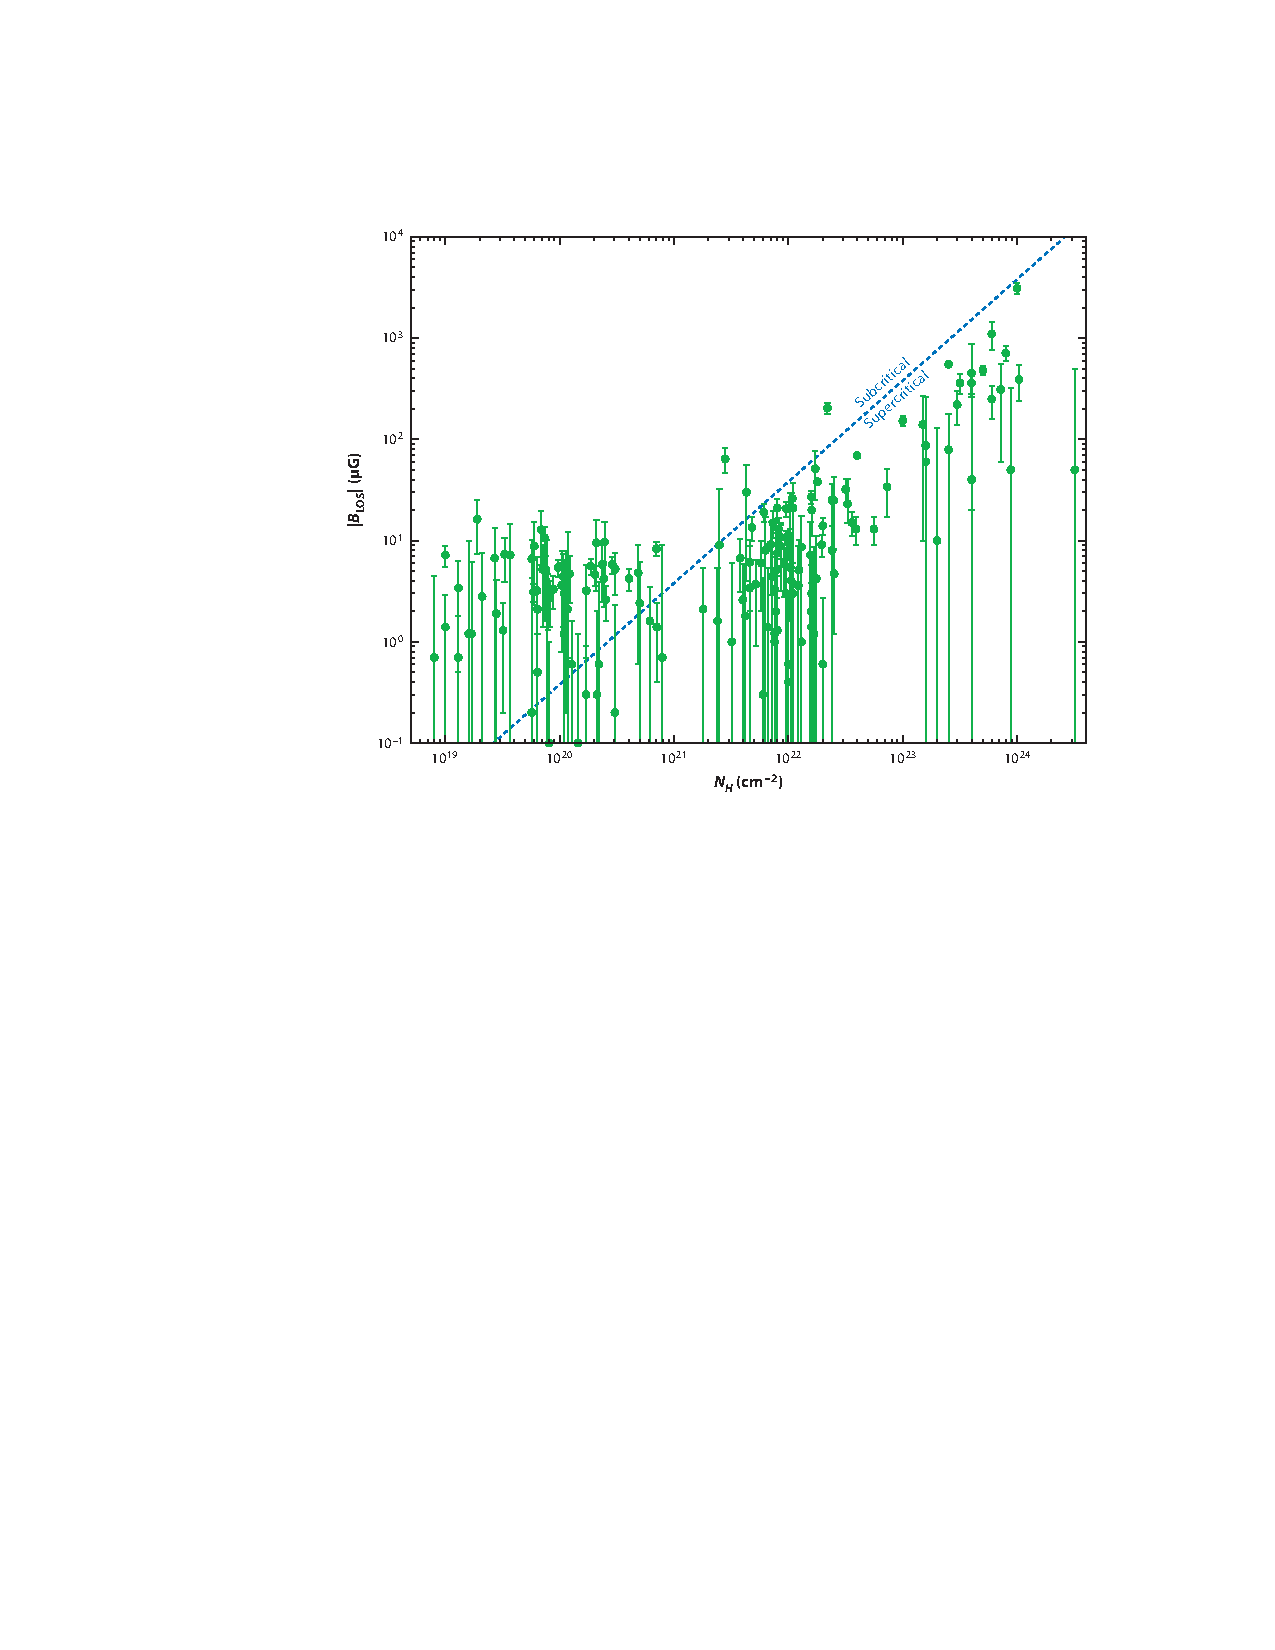
\includegraphics[width=\linewidth]{bfields_crutcher12}
\caption[Magnetic field strength measurements]{
\label{fig:bfields}
Measurements of the line of sight magnetic field strength from the Zeeman effect, versus total gas column density in H atoms cm$^{-2}$ (data from the compilation of \citealt{crutcher12a}). The three clumps of points represent, from left to right, measurements from the Zeeman splitting of H~\textsc{i}, OH, and CN. The dashed black line indicates the separation between field strengths that are large enough to render the gas subcritical, and those weak enough for it to be supercritical.
}
\end{figure}

\subsection{Turbulent Support}

There is one more positive term in the virial theorem, which is the turbulent component of $\mathcal{T}$. This one is not at all well understood, largely because we don't understand turbulence itself. This term almost certainly provides some support against collapse, but the amount is not well understood, and we will defer any further discussion of this effect until we get to our discussions of the star formation rate in Chapter \ref{ch:sflaw_th}.

\section{Pressureless Collapse}
\label{sec:pressureless_collapse}

As a final topic for this chapter, let us consider what we should expect to happen if gas does begin to collapse, in the simplest case of an initially-spherical cloud with an initial density distribution $\rho(r)$. We would like to know how the gas moves under the influence of gravity and thermal pressure, under the assumption of spherical symmetry. For convenience we define the enclosed mass
\begin{equation}
M_r =  \int_0^r 4\pi r'^2 \rho(r') \, dr'
\end{equation}
or equivalently
\begin{equation}
\frac{\partial M_r}{\partial r} = 4\pi r^2 \rho.
\end{equation}
The equation of mass conservation for the gas in spherical coordinates is
\begin{eqnarray}
\frac{\partial}{\partial t} \rho + \nabla\cdot (\rho \vecv) & = & 0 \\
\frac{\partial}{\partial t} \rho + \frac{1}{r^2}\frac{\partial}{\partial r}(r^2 \rho v) & = & 0,
\end{eqnarray}
where $v$ is the radial velocity of the gas. It is useful to write the equations in terms of $M_r$ rather than $\rho$, so we take the time derivative of $M_r$ to get
\begin{eqnarray}
\frac{\partial}{\partial t}M_r & = & 4\pi \int_{0}^{r} r'^2 \frac{\partial}{\partial t} \rho \,dr' \\
& = & -4\pi \int_{0}^{r} \frac{\partial}{\partial r'}(r'^2 \rho v)\, dr' \\
& = & -4\pi r^2 \rho v \\
& = & -v \frac{\partial}{\partial r}M_r.
\end{eqnarray}
In the second step we used the mass conservation equation to substitute for $\partial \rho/\partial t$, and in the final step we used the definition of $M_r$ to substitute for $\rho$.

To figure out how the gas moves, we write down the Lagrangean version of the momentum equation:
\begin{equation}
\rho \frac{Dv}{Dt} = -\frac{\partial}{\partial r}P - \mathbf{f}_g,
\end{equation}
where $\mathbf{f}_g$ is the gravitational force. For the momentum equation, we take advantage of the fact that the gas is isothermal to write $P=\rho c_s^2$. The gravitational force is $\mathbf{f}_g = -G M_r / r^2$. Thus we have
\begin{equation}
\frac{Dv}{Dt}= \frac{\partial}{\partial t}v + v\frac{\partial}{\partial r} v= -\frac{c_s^2}{\rho} \frac{\partial}{\partial r}{\rho} - \frac{G M_r}{r^2}.
\end{equation}

To go further, let us make one more simplifying assumption: that the sound speed $c_s$ is zero. This is not as bad an approximation as one might think. Consider the virial theorem: the thermal pressure term is just proportional to the mass, since the gas sound speed stays about constant. On the other hand, the gravitational term varies as $1/R$. Thus, even if pressure starts out competitive with gravity, as the core collapses the dominance of gravity will increase, and before too long the collapse will resemble a pressureless one.

In this case the momentum equation is trivial:
\begin{equation}
\frac{Dv}{Dt} = -\frac{GM_r}{r^2}.
\end{equation}
This just says that a shell's inward acceleration is equal to the gravitational force per unit mass exerted by all the mass interior to it, which is constant. We can then solve for the velocity as a function of position:
\begin{equation}
v = \dot{r} = -\sqrt{2GM_r}\left(\frac{1}{r}-\frac{1}{r_0}\right)^{1/2},
\end{equation}
where $r_0$ is the position at which a particular fluid element starts. 

The integral can be evaluated by the trigonometric substitution $r=r_0 \cos^2\xi$. The solution, first obtained by Hunter (1962), is
\begin{eqnarray}
-2 r_0 (\cos\xi \sin\xi) \dot{\xi} & = & -\sqrt{\frac{2GM_r}{r_0}} \left(\frac{1}{\cos^2\xi}-1\right)^{1/2} \\
2 (\cos\xi\sin\xi) \dot{\xi} & = & \sqrt{\frac{2GM_r}{r_0^3}}\tan\xi \\
2 \cos^2\xi\, d\xi & = & \sqrt{\frac{2GM_r}{r_0^3}} dt \\
\xi+\frac{1}{2}\sin 2\xi & = & t \sqrt{\frac{2GM_r}{r_0^3}}.
\end{eqnarray}
We are interested in the time at which a given fluid element reaches the origin, $r=0$. This corresponds to $\xi = \pi/2$, so this time is
\begin{equation}
t = \frac{\pi}{2}\sqrt{\frac{r_0^3}{2 G M_r}}.
\end{equation}

Suppose that the gas we started with was of uniform density $\rho$, so that $M_r = (4/3)\pi r_0^3 \rho$.
In this case we have
\begin{equation}
t = t_{\rm ff} = \sqrt{\frac{3\pi}{32 G \rho}},
\end{equation}
where we have defined the free-fall time $t_{\rm ff}$: it is the time required for a uniform sphere of pressureless gas to collapse to infinite density. This is of course just the characteristic growth time for the Jeans instability in the regime of negligible pressure, up to a factor of order unity.

For a uniform fluid this means that the collapse is synchronized -- all the mass reaches the origin at the exact same time. A more realistic case is for the initial state to have some level of central concentration, so that the initial density rises inward. Let us take the initial density profile to be $\rho = \rho_c (r/r_c)^{-\alpha}$, where $\alpha > 0$ so the density rises inward. The corresponding enclosed mass is
\begin{equation}
M_r = \frac{4}{3-\alpha}\pi \rho_c r_c^3 \left(\frac{r}{r_c}\right)^{3-\alpha} 
\end{equation}

Plugging this in, the collapse time is
\begin{equation}
t = \sqrt{\frac{(3-\alpha)\pi}{32 G \rho_c}} \left(\frac{r_0}{r_c}\right)^{\alpha/2}.
\end{equation}
Since $\alpha>0$, this means that the collapse time increases with initial radius $r_0$. This illustrates one of the most basic features of a collapse, which will continue to hold even in the case where the pressure is non-zero. Collapse of centrally concentrated objects occurs inside-out, meaning that the inner parts collapse before the outer parts.

Within the collapsing region near the star, the density profile also approaches a characteristic shape. If the radius of a given fluid element $r$ is much smaller than its initial radius $r_0$, then its velocity is roughly
\begin{equation}
v \approx v_{\rm ff}\equiv -\sqrt{\frac{2GM_r}{r}},
\end{equation}
where we have defined the free-fall velocity $v_{\rm ff}$ as the characteristic speed achieved by an object collapsing freely onto a mass $M_r$. The mass conservation equation is
\begin{equation}
\frac{\partial M_r}{\partial t} = -v\frac{\partial M_r}{\partial r}  = -4\pi r^2 v \rho
\end{equation}

If we are near the star so that $v\approx v_{\rm ff}$, then this implies that
\begin{equation}
\rho = \frac{(\partial M_r/\partial t) r^{-3/2}}{4\pi\sqrt{2 G M_r}}.
\end{equation}
To the extent that we look at a short interval of time, over which the accretion rate does not change much (so that $\partial M_r /\partial t$ is roughly constant), this implies that the density near the star varies as $\rho\propto r^{-3/2}$.

What sort of accretion rate do we expect from a collapse like this? For a core of mass $M_c = [4/(3-\alpha)]\pi \rho_c r_c^3$, the last mass element arrives at the center at a time
\begin{equation}
t_c = \sqrt{\frac{(3-\alpha)\pi}{32 G \rho_c}} = \sqrt{\frac{3-\alpha}{3}}t_{\rm ff}(\rho_c),
\end{equation}
so the time-averaged accretion rate is
\begin{equation}
\langle\dot{M}\rangle = \sqrt{\frac{3}{3-\alpha}} \frac{M_c}{t_{\rm ff}(\rho_c)}.
\end{equation}

In order to get a sense of the numerical value of this, let us suppose that our collapsing object is a marginally unstable Bonnor-Ebert sphere (see Problem Set 2). Such an object does not have negligible pressure, but the pressure will only change the collapse rate at order unity. Problem Set 2 includes a calculation of the structure of a maximum-mass Bonnor-Ebert sphere, so we will just quote the value. The maximum mass is
\begin{equation}
M_{\rm BE} = 1.18 \frac{c_s^4}{\sqrt{G^3 P_s}},
\end{equation}
where $P_s$ is the pressure at the surface of the sphere and $c_s$ is the thermal sound speed in the core.

Let us suppose that the surface of the core, at radius $r_c$, is in thermal pressure balance with its surroundings. Thus $P_s = \rho_c c_s^2$, so we may rewrite the Bonnor-Ebert mass as
\begin{equation}
M_{\rm BE} = 1.18 \frac{c_s^3}{\sqrt{G^3 \rho_c}}.
\end{equation}
A Bonnor-Ebert sphere does not have a powerlaw structure, but if we substitute into our equation for the accretion rate and say that the factor of $\sqrt{3/(3-\alpha)}$ is a number of order unity, we find that the accretion rate is
\begin{equation}
\langle\dot{M}\rangle \approx \frac{c_s^3/\sqrt{G^3\rho_c}}{1/\sqrt{G\rho_c}} = \frac{c_s^3}{G}.
\end{equation}

This is an extremely useful expression, because we know the sound speed $c_s$ from microphysics. Thus, we have calculated the rough accretion rate we expect to be associated with the collapse of any object that is marginally stable based on thermal pressure support. Plugging in $c_s=0.19$ km s$^{-1}$, we get $\dot{M} \approx 2\times 10^{-6}$ $\msun$ yr$^{-1}$ as the characteristic accretion rate for these objects. Since the typical stellar mass is a few tenths of $\msun$, based on the peak of the IMF, this means that the characteristic star formation time is of order $10^5-10^6$ yr. Of course this conclusion about the accretion rate only applies to collapsing objects that are supported mostly by thermal pressure. Other sources of support produce higher accretion rates, as we will see when we get to massive stars.


